\documentclass[11pt]{article}

\usepackage{setspace}
\usepackage[margin=1.75in]{geometry}

% Make table of contents look better
\usepackage{tabularx}
\usepackage{tocloft}
\renewcommand{\cftsecleader}{\cftdotfill{\cftdotsep}}

\usepackage{graphicx}
\usepackage{pdfpages}
\usepackage{hyperref}

% \usepackage[ngerman]{babel}
% \usepackage[T1]{fontenc}
% \usepackage[ansinew]{inputenc}
% \usepackage{lmodern}

% Times New Roman font
\usepackage{txfonts}

\begin{document}

\setlength{\parindent}{2em}

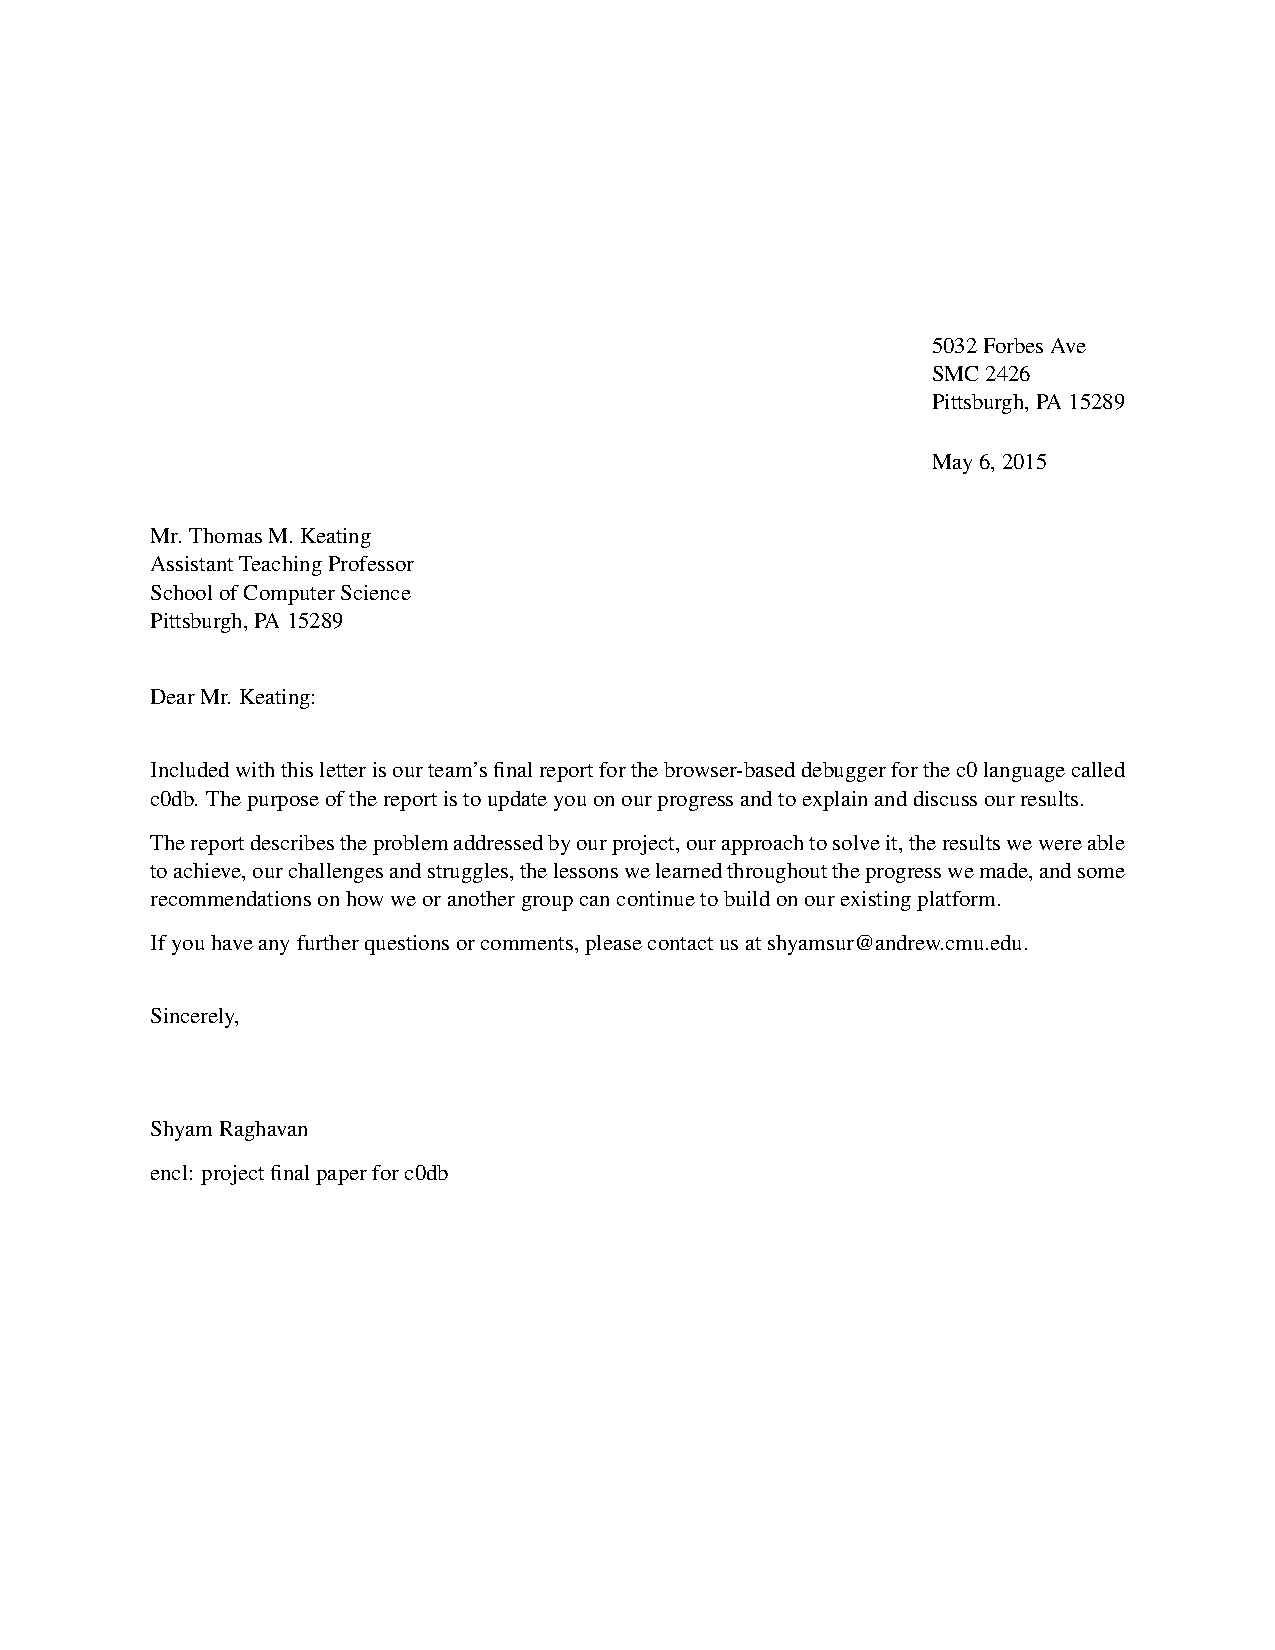
\includepdf[pages={1}]{letter.pdf}

\begin{titlepage}
\clearpage
\thispagestyle{empty}

\begin{center}
{\Huge Final Report}\\
\vspace{10 mm}
{\Huge {\tt c0db}\\[.4em]
The {\tt C0} Debugger}\\
\vspace{10 mm}

Submitted to\\
Mr. Thomas M. Keating\\
Assistant Teaching Professor\\
School of Computer Science\\
Carnegie Mellon University\\
Pittsbugh, PA 15289

\vspace{10 mm}

Prepared by:\\
{\bf Aaron Gutierrez}\\
{\bf Shyam Raghavan}\\
Mitchell Plamann\\
Suhaas Reddy

\vspace{10 mm}

School of Computer Science\\
Carnegie Mellon University\\
\today

\vspace{10 mm}

{\bf Abstract}
\end{center}
\par
Finding problems in code is a difficult and time consuming task, one especially
difficult for programmers learning a new language. To help students more quickly
find bugs and understand how their programs run, we created an online debugger
for the {\tt C0} programming language. The {\tt C0} debugger, {\tt c0db},
enables users to run programs in their browser and break apart the execution
when they don't run correctly.
\end{titlepage}

\pagenumbering{roman}
\tableofcontents
\newpage

\pagenumbering{arabic}

\section{Introduction}
We discuss the problems we hoped to resolve, give an overview of the project,
and show how the project solves the problems outlined. We also analyze the
effectiveness of the literature reviewed and the final accomplishments compared
to our original goals.
\subsection{Background}
One of Carnegie Mellon University's most widely attended class is 15-122,
Principles of Imperative Computation. 15-122 contains a capstone assignment
called the {\tt C0} Virtual Machine, which involves implementing a program that
allows the user to run arbitrary code in the language in which 15-122 is
taught, {\tt C0}. The implementation of the virtual machine (C0VM) is not an
easy task - it involves higher level thinking and a deep understanding of the
abstractions associated with running arbitrary code.
\par
Because it is difficult, the {\tt c0db} ({\tt C0} Debugger) hoped to improve
the learning process by making visualization and interaction with a working
implementation of the C0VM more accessible to 15-122 students. This involved
creating a working Javascript version of the C0VM, implementing visualizers for
relevant parts of the assignment, and developing the interface for
student-based interaction with the application.
\par
In order to begin learning using {\tt C0}, students must
become familiar with the Unix operating system environment. This overhead
causes a delay in the learning of students, and increases the barrier to entry
for many people.
\subsection{Project Overview}
By implementing the {\tt c0db}, we hoped to benefit students in 15-122 by
helping them create correct programs. The {\tt c0db} will enable students to
understand how their programs execute and find where problems originate more
easily than with existing tools. In addition to debugging, students will have a
more familiar understanding of the underlying computational model represented
in the debugger through the use of our application.
\par
The {\tt C0} Debugger will also enable students to test simple programs with
little setup, using only a web browser. They will no longer have to set up and
become familiar with a Unix environment before they can program, making {\tt
C0} accessible to more people.
\par
The project manifested itself in what is now \url{http://c0db.herokuapp.com}.
The application provides an input field for students to enter {\tt C0} code,
outputs intermediate bytecode, and has the ability to run said bytecode. The
application also has functionality that allows for breakpoints, stepping
through code, and continuing the code from the current breakpoint. With this
application, we were able to effectively meet the goals of improving coding
accessibility, creating familiarity with the underlying computational model of
computers, and being able to more easily debug programs. We were unable to
effectively meet the goals of visualization and interactivity with respect to
the debugger and {\tt C0}.
\subsection{Analysis of Literature Review}
There was very little relevant literature to the subject at hand. The
documentation found involved implementing Javascript virtual machines and
debuggers, and while this was of some use (detailed below), the disconnect
between implementing a Javascript virtual machine and a {\tt C0} virtual
machine was apparent. This was also felt in the literature associated with
processing user-input code.
\par
The literature that was discovered during development became very helpful as
the project evolved. Of particular importance was unit testing and the original
handout given to students implementing the virtual machine in C.
\par
The greatest difficulties faced by the lack of information pertaining to
creating a virtual machine for a language that was not Javascript involved
developing the framework to parse through the intermediate bytecode given
by the compiler of {\tt C0}. The information about building an in-browser
Javascript VM and debugger\footnote{http://amasad.me/2014/01/06/building-an-in-browser-javascript-vm-and-debugger-using-generators/}
was a particular example of this. We hoped to design our debugger's architecture
based on this virtual machine's architecture. The literature mentioned being
designed in two parts. Specifically, the application was designed around a
virtual machine and a debugger. Unfortunately, because of the way {\tt C0} is
designed and the way the bytecode intermediate is evaluated, we found it very
difficult to follow this modularized approach, and had to combine the two.
\par
The second piece of literature we believed would be helpful when proposing this
project\footnote{http://www.aosabook.org/en/pjs.html} was not helpful at all.
While it did give us issues to consider such as the lack of threading and the
presence of asynchronous calls in Javascript, we felt as though it did not
provide any information about the transferral of information from the webpage
to the back-end virtual machine and debugger. This was what we hoped we would
be able to use from it, and while it was helpful in giving ideas about possible
approaches to this problem, it did not give any insight into the development of
a script to compile code and receive intermediate bytecode (the solution that
we eventually employed).
\par
The other pieces of literature we reviewed (the Node.js
documentation\footnote{http://nodejs.org/documentation/}, the Nodeunit
documentation\footnote{https://github.com/caolan/nodeunit}, and the handout
given to students to complete the {\tt C0} virtual
machine\footnote{https://www.cs.cmu.edu/~rjsimmon/15122-f14/prog/c0vm-writeup.pdf})
were all very helpful. The handout helped us design an architecture that
allowed for easy implementation in the browser and in Javascript. This
architecture was very similar to that of the architecture that students are
given when first completing the virtual machine in C. The Node.js documentation
and Nodeunit documentation proved very useful when developing the application
and creating unit tests to test the framework and the application. The
documentation provided easy answers to questions that arose with implementation.
\subsection{Successes}
The final product was successful at completing three of the four goals we set
out to accomplish. We were successful at improving accessibility of coding and
programming to students and beginners. The application allows for a simple
interface to enter code, compile it, and run it. We were successful at
creating familiarity with the underlying computation model represented in a
virtual machine. The application gives information about the current state
of the model at each point in execution, and allows the user to examine the
internals of the computational model. Finally, we were also successful at
creating a tool that allows for debugging {\tt C0} code. This is represented
in the ability of the application to step through the code.
\par
We were not successful at developing a visualization component to help
beginners learn about the computational model. This is something we hope to
be able to do and, in the future, we hope will help the students of 15-122
learn more about computer science.

\section{Approach}
In this section, we outline the various phases of our development cycle. We
also make note of the technologies used to implement the application.

\begin{figure}[h]
  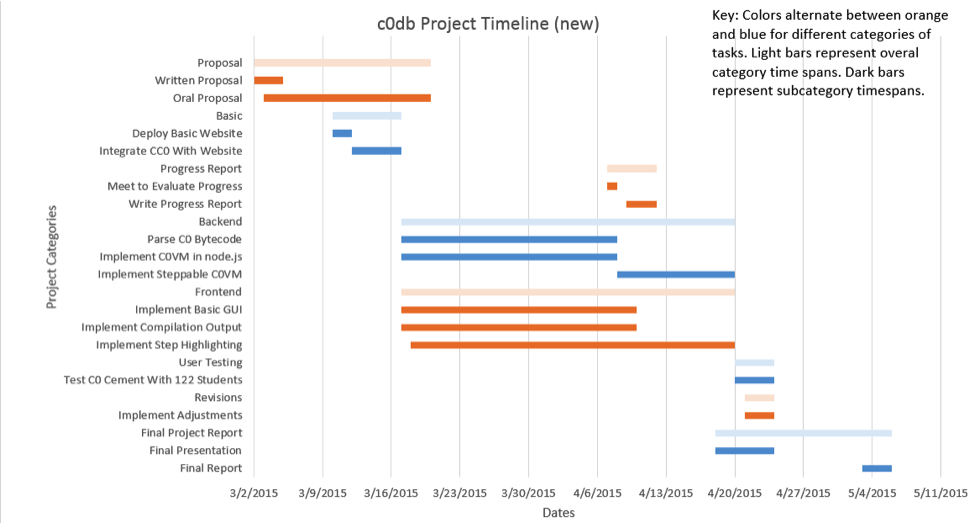
\includegraphics[width=\linewidth]{new-gantt}
  \caption{Revised project Gantt chart}
  \label{gantt}
\end{figure}
\subsection{Phase 1}
Phase 1 was centered around the design of the application, and didn't involve
very much actual programming. This phase was completed a bit later than hoped.
However, due to its short nature, it did not put us far behind our ideal
schedule. During Phase 1, we realized that the best option for architecture
of our application was to structure it similarly to the structure that students
in 15-122 use and that is provided by the course staff.
\par
While the infrastructure could have been designed in a more efficient way, we
feel as though Phase 1 was effective at creating a base layer from which to
implement both the front-end and the back-end of the application. At the end
of Phase 1, we had a framework upon which the successful web application was
developed, and we were able to coordinate and delegate tasks between team
members.
\subsection{Phase 2}
Phase 2 was focused on the back-end of the application. Phase 2 involved
actually implementing the framework described in Phase 1, developing the script
to transform uncompiled {\tt C0} code into bytecode intermediate, developing
the virtual machine in which the bytecode was executed, implementing a
state-based breakpoint system that allows for inserting breakpoints into the
code, and implementing step-based functionality that allows for users to step
through the running code.
\par
In this phase, we used the Node.js framework to implement the application. This
framework is a commonly-used web application framework in Javascript that is
used to easily get a running website. We also found Nodeunit, a unit testing
framework designed for use with the Node.js framework. Nodeunit allowed us to
write over 50 test files to check for correctness and safety of our virtual
machine.
\par
This phase finished on time after the revision of the Gantt chart (\ref{gantt}).
There are still some features that we would like to implement before declaring
the back-end finished, but these involve going further than the stated goals.
The back-end created an effective interface from which the front-end team was
able to develop the front-end.
\subsection{Phase 3}
Phase 3 was focused on the front-end of the application. Phase 3 involved
implementing the front-end side of the framework described in Phase 1. This
includes implementing the user interface for inputting {\tt C0} code, creating
the design and implementing the design for outputting the intermediate
bytecode, creating an effective medium of outputting runtime output, and
developing an interactive suite of tools for debugging such as adding
breakpoints, stepping through code, and viewing the internal computational
model.
\par
In this phase, we used LESS, a CSS preprocessor, as opposed to plain CSS. LESS
is a widely used styling language that is compiled into CSS because it is easier
to write than CSS. We also used JQuery, a front-end framework that is used to
connect elements of the front-end design to back-end Javascript. These were
chosen because they allow for fast, correct development, and make it easier
to focus on development and design, not rewriting existing code.
\par
This phase also finished on time after the revision of the Gantt chart
(\ref{gantt}). We did not quite finish all features we hoped we would be able
to complete originally. The features not completed involved more intuitive
interactivity and a better visualization tool for viewing the internals of the
computational model. The front-end, however, was successful at developing the
front-end such that most desired goals were achieved.
\subsection{Phases 4 and 5}
Phases 4 and 5 were centered around user testing and revision. These phases
are still in process, and will continue to be in process until the tool is
developed to the point at which it is used in the 15-122 course curriculum.
Phase 4 involved showing the product to the 15-122 course staff and getting
opinions from the teaching assistants that would be using the tool in a
teaching setting, showing the product to the 15-122 professors, and showing
the product to 15-122 students. Each of these groups was given an opportunity
to interact with the product, and was asked to provide feedback on usability,
learnability, and overall usefulness. Phase 5 involves revising the product
based on this feedback. Phase 4 is still in process, and as a result, Phase 5
has not begun yet.

\section{Results}
We originally aimed to evaluate our performance against user feedback from both
current and past students. However, due to setbacks in the early stages of
development we were unable to receive significant use feedback from students.
That said, we were able to gather feedback and support from current 15-122
course staff.
\par
In terms of our original vision, {\tt c0db} includes almost every feature we
planned to implement. Users can input code and either run the program straight
through or step through execution instruction by instruction. The only
significant feature that is not currently implemented completely is breakpoints.
Implementing breakpoints turned out to be significantly more difficult than we
anticipated, and given our limited time frame, we were unable to come up with an
adequate solution. We are currently working with Rob Simmons, 15-122 instructor
and maintainer for the {\tt C0} language standard, to extend the language to
support breakpoints more easily going forward.

\begin{figure}[h]
  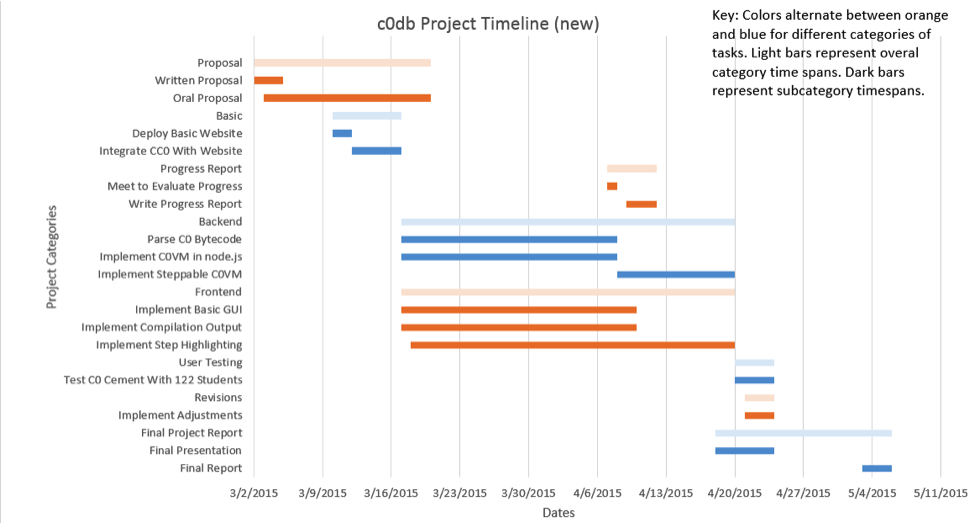
\includegraphics[width=\linewidth]{new-gantt}
  \caption{Revised project Gantt chart (copied from above for convenience)}
  \label{gantt}
\end{figure}
Relative to our revised Gantt Chart (Figure \ref{gantt}) we hit every milestone
on time. Both the front-end and back-end teams completed their tasks by the end
of April, at which point we transitioned everyone to user testing, revisions,
and polishing. Both teams were able to recover from the lag reported in our
progress report to complete {\tt c0db}.

\section{Discussion}
\subsection{Reflection}
Our team learned several useful skills while working on this project, ranging
from technical tricks to communication insights. For several of us, this project
represents the most collaboration on a single code base. We effectively employed
the git version control system to manage our code to lesson the work needed to
integrate each person's features. Additionally, several members of our team had
never worked with node.js or JavaScript extensively before this project.
Everyone quickly picked up the new framework and started producing useful
output.
\par
We did face some issues communicating early on, but fortunately we were able to
learn from our problems. Communicating strictly online was not sufficient and
resulted in a lack of ownership and drive that put us behind schedule early on.
We overcame our communication problems by holding brief but regular meetings
face to face to cover what has been accomplished and what tasks come next.

\subsection{Future}
{\tt C0db} is most of what we imagined, but not all. Our overall goal, to make a
tool useful for 15-122 students, may be realized in the fall, but we have more
work to ensure that we present them with the best tool possible. Before the next
semester starts we aim to complete the remaining features we originally planned
to implement: source-level breakpoints, multi-file support, and a refined
interface. If we can implement these three features, {\tt c0db} could see proper
adoption by 15-122 in the fall, where it would be used by over 300 students from
across Carnegie Mellon. If {\tt c0db} is adopted by 15-122, we would truly have
achieved the goal for our project: create a tool to better the CMU community.

\section{Sources Cited}
\begin{enumerate}
\item Amjad Masad,
  ``Building an In-Browser JavaScript VM and Debugger Using Generators'',
  http://amasad.me/2014/01/06/building-an-in-browser-javascript-vm-and-debugger-using-generators/
\item Mike Kamermans, ``The Architecture of Open Source Applications (Volume 2)'',
  http://www.aosabook.org/en/pjs.html
\item Joyent, Inc., ``Node.js Documentation'',
  http://nodejs.org/documentation
\item ``Nodeunit documentation'',
    https://github.com/caolan/nodeunit
\item ``c0vm Assignment Handout'',\\
    https://www.cs.cmu.edu/~rjsimmon/15122-f14/prog/c0vm-writeup.pdf
\end{enumerate}

\end{document}
